\documentclass[12pt,twocolumn]{article}
\usepackage[utf8]{inputenc}
\usepackage[english]{babel}
\usepackage[table,xcdraw]{xcolor}
\usepackage{physics}
\usepackage{fancyhdr}
\usepackage{geometry}
\usepackage{natbib}
\usepackage{graphicx}
\usepackage{float}
\usepackage{wrapfig}
%\usepackage{caption}
\usepackage[justification=centering]{caption}
\usepackage{subcaption}
\usepackage{gensymb}
\usepackage[export]{adjustbox}
\usepackage{hyperref}
\geometry{margin = 20mm}
\usepackage{mathtools}
\usepackage{amsmath}
\usepackage{indentfirst}
\usepackage{xurl}
\usepackage{t1enc}
\usepackage{setspace}


\title{Simulating detectors with Geant4 4th report}
\author{Scientific Modeling Computer Laboratory\\Bendegúz Borkovits T7UR9P\\Supervisor: Ákos Horváth}
\date{April 2022}


\begin{document}

\maketitle

\section{Introduction}

Last time, the process of working with Geant4 came to a halt, since there arose an error upon launching the simulation. However, after receiving help and advice from the creator of the simulation, Balázs Pál, the error has been corrected. \cite{masterdesky} Thus, the continuation of the project was assured.

This report contains the results that were gained after running the NEBULA simulation with given parameters. These results consist of the relative number of particles organized by particle type, generating process type and volume type, the last of which means the target module the particles were detected at. The analysis was done in python and all the resulting files as well as the simulation can be located in my github repository. \cite{borbende}

\section{Parameters}

One two-layered wall of the NEBULA consists of sixty NEUT and twelve VETO modules of which, here only eighteen neutron detectors are modelled. \cite{nebula} To generate the required data, a neutron beam that consisted of one hundred particles with 100 MeV initial energy was projected onto the wall. This process is shown on Figure 1. After the beam interacts with the various modules in the wall, multiple events occur like ionization, elastic scattering, back scattering and so forth. Numerous new particles are detected in the process like protons, deuterons, or photons. Due to this, a problem has arisen with the visualization. Although, Geant4 provides an excellent visualization tool for our experiments, even it has its limit in distinguishing all the different types of by-product particles. There are some methods to make the output more pleasing to the eye, however in this case, it might not work due to the large number of particle types.
\begin{figure}[H]
    \centering
    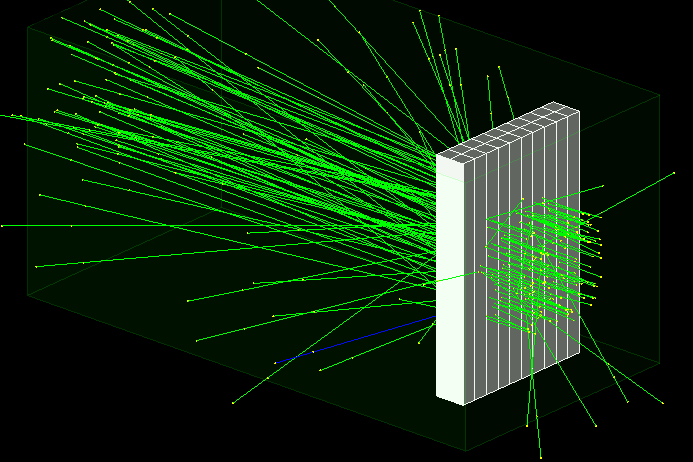
\includegraphics[scale = 0.5]{qbbc_neutbeam.png}
    \caption{Showcasing the trajectory of the neutron beam.}
    \label{fig:my_label}
\end{figure}
One might ask, what kind of physics lists would the measurement of neutrons require. For this purpose, Geant4 offers a great deal of choices. \cite{geant} This is rather joyous news, since it is our task to examine the output of the simulation using various physics lists. The lists chosen for this simulation are the following. Four different lists of the QGSP physics list library that stands for Quark Gluon String Physics and works around said model. These are BERT\_HP that uses the Geant4 Bertini Cascade, BIC\_HP that uses the Binary light Ion Cascade, INCLXX that revolves around the Liege Intranuclear Cascade model, and INCLXX\_HP that is similar to the earlier mentioned one but also includes the data driven high precision neutron package (HP). \cite{geant}

\section{Results}
After running the simulation once for every physics list, we obtained the figures that are shown in the appendix of this document. The relative number of particles means the number of particles rendered to a given category in the histogram, like number of protons or number of particles detected by the fourteenth NEUT module.

When we categorize the number of particles by their type, it is shown on Figure 2 that the protons generated by the interaction between the beam and the detector is the highest or is almost equal to the number of neutrons present. This behaviour reappears on all five subplots. It is because of these results, that we show no surprise when realizing upon looking at Figure 3 that the dominant particle generating processes during the simulation were hadronic processes. Then, when taking a look at the number of particles detected by the different modules, it is shown on Figure 4 that the corners on the wall, that consist of Counter1, 2, 16 and 17 detected the least of them as expected.

Upon measuring and plotting the deposited energy, I sorted the values in descending order to have a better view of the situation. The protons were shown to have the largest amount of deposited energy on Figure 5. Unsurprisingly, the already determined most dominant hadronic ionization process was detected to be dominant in energy as well, as it was showcased on Figure 6. Finally on Figure 7, we noticed that there are quite a few differences between the order of Counters on the different subplots. However, this is only due to the fact that the difference in energy between many Counters is negligible and thus prone to change with randomness during each run. Also, it does not come as a surprise that the energy deposited to the world volumes is significantly less than those deposited to the modules.

\section{Discussion}
The goals for the past two weeks have been to run the simulation using neutrons with 100 MeV as initial energy, acquire the deposited energy and check its value for each NEUT module. These conditions have been met and have been expanded upon by including several categorizations for the number of detected particles and deposited energy. These computations were applied to the simulation using various physics lists which was another task for this period of time.

For the last two weeks a reasonable goal would be to try and measure the detector efficiency by generating data of the deposited energy for numerous initial energies.

\bibliographystyle{plain}
\bibliography{references.bib}




\onecolumn
\section*{Appendix}

\begin{figure}[H]
    \centering
    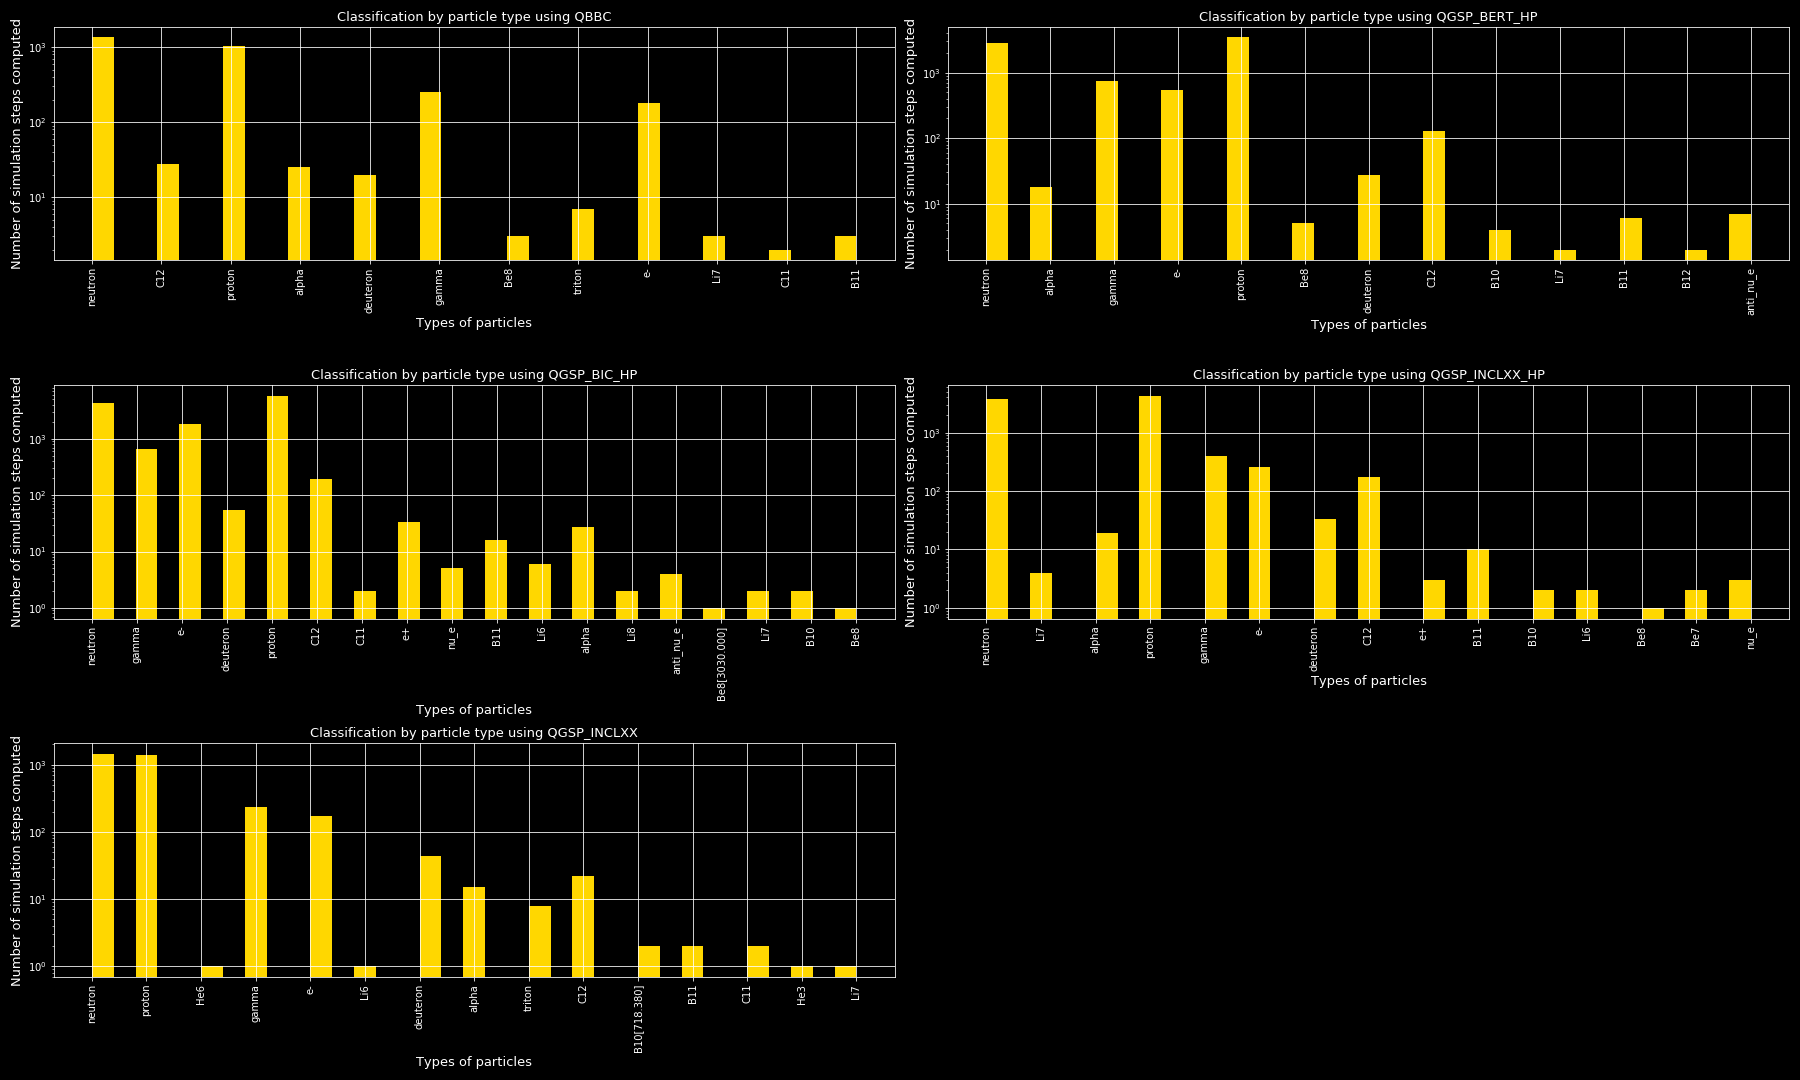
\includegraphics[scale = 0.25]{numparticles.png}
    \caption{Summing the relative number of particles by their types.}
    \label{fig:my_label}
\end{figure}

\begin{figure}[H]
    \centering
    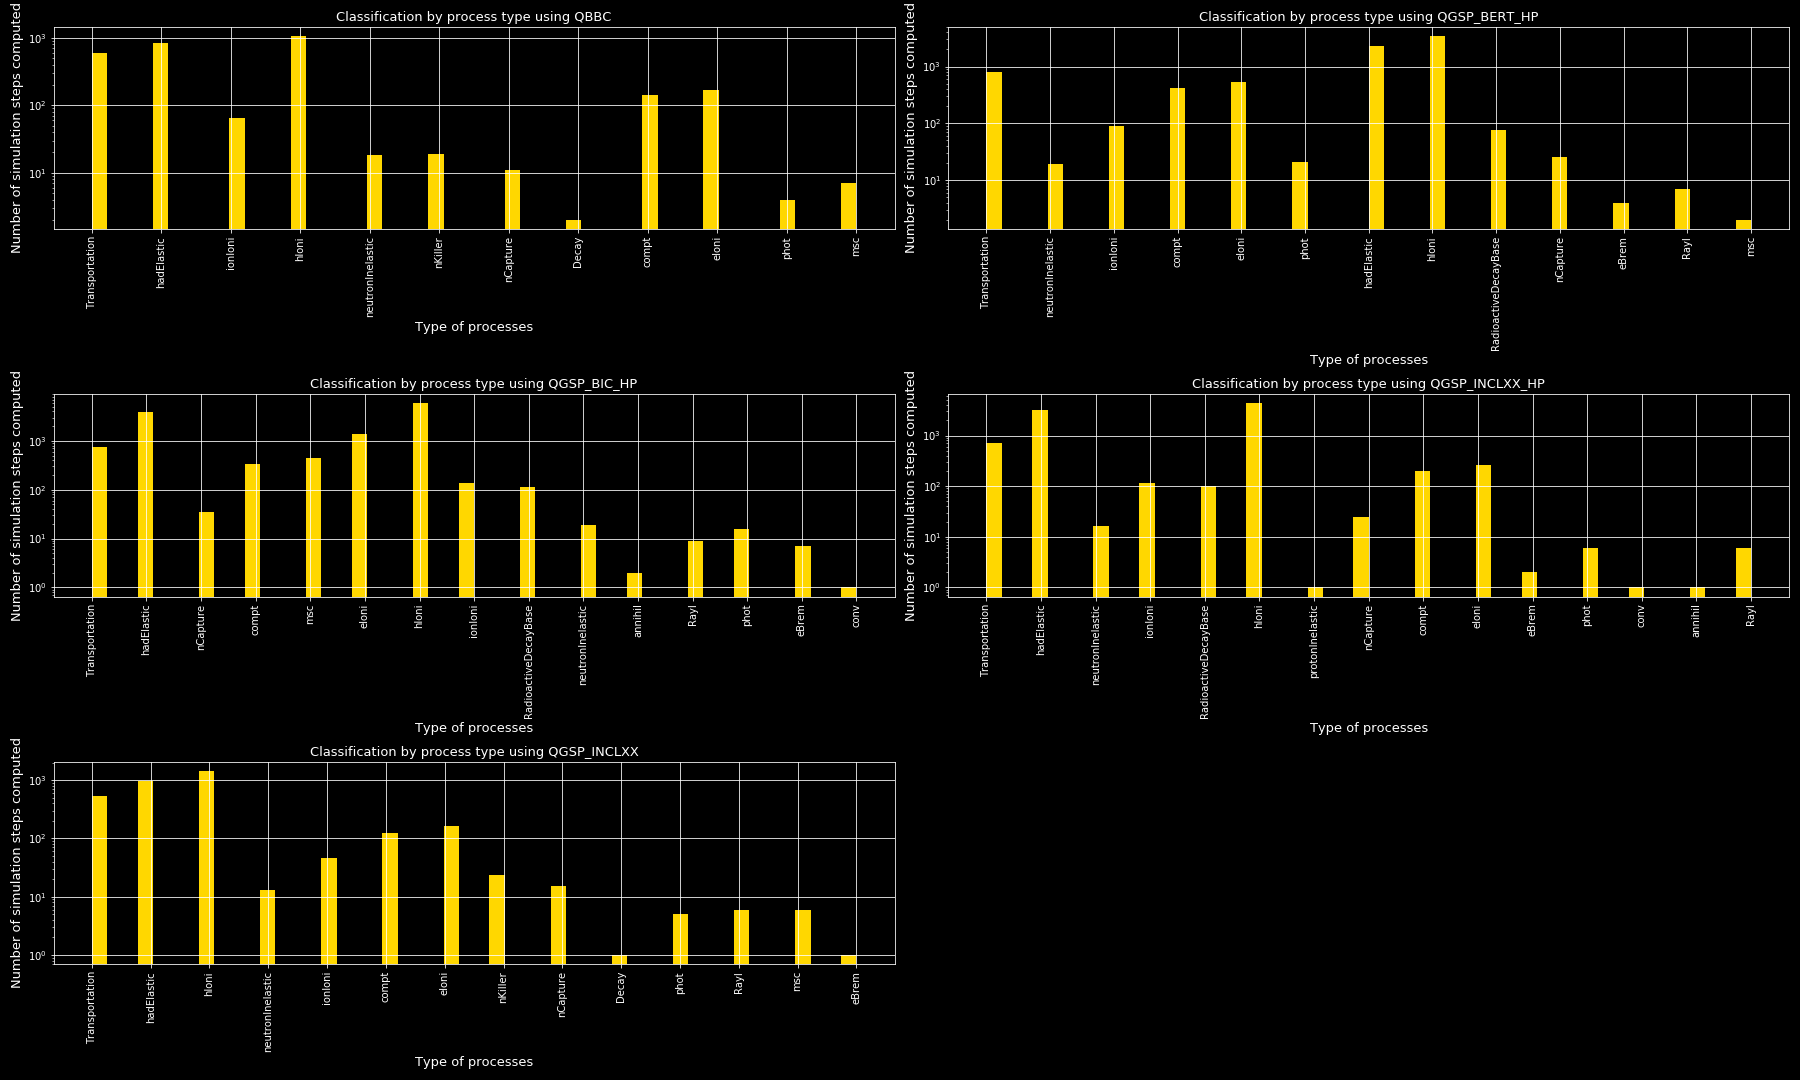
\includegraphics[scale = 0.25]{numprocess.png}
    \caption{Summing the relative number of particles by the processes that generated them.}
    \label{fig:my_label}
\end{figure}

\begin{figure}[H]
    \centering
    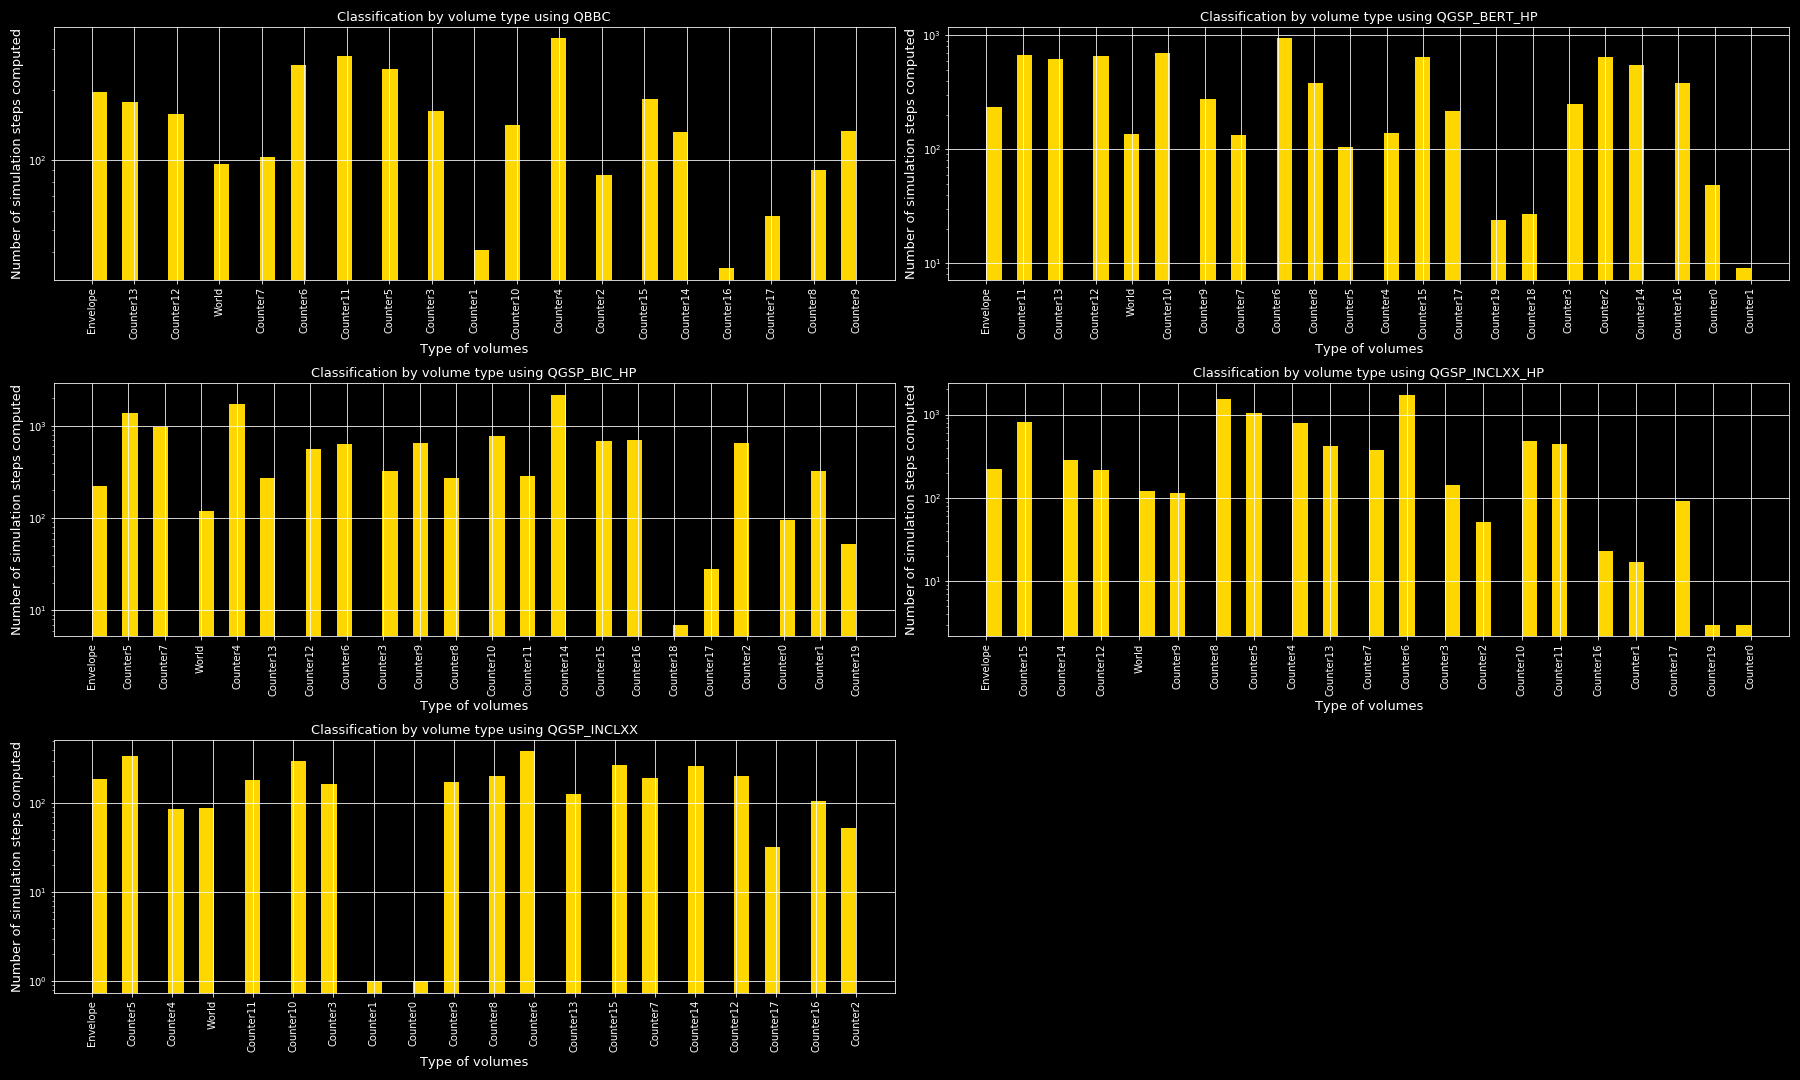
\includegraphics[scale = 0.25]{numvolumes.png}
    \caption{Summing the relative number of particles by the volumes they were detected in.}
    \label{fig:my_label}
\end{figure}

\begin{figure}[H]
    \centering
    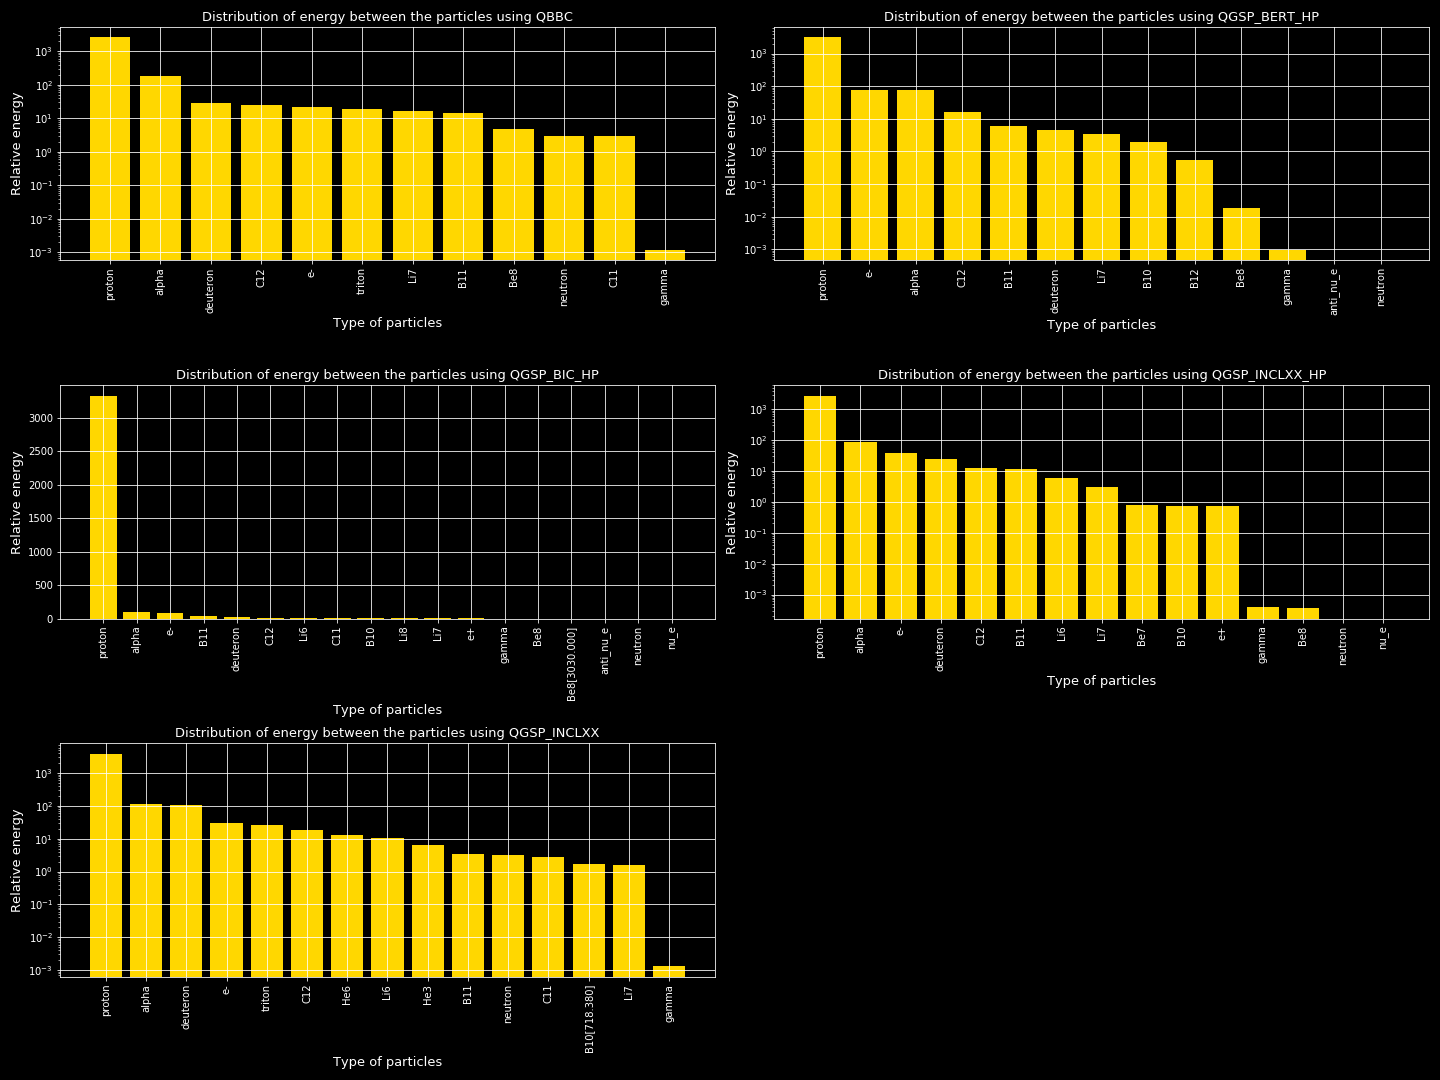
\includegraphics[scale = 0.30]{enpart.png}
    \caption{Summing the relative energy distributed among the particles by particle type. The log scale of the third subplot was bugged.}
    \label{fig:my_label}
\end{figure}

\begin{figure}[H]
    \centering
    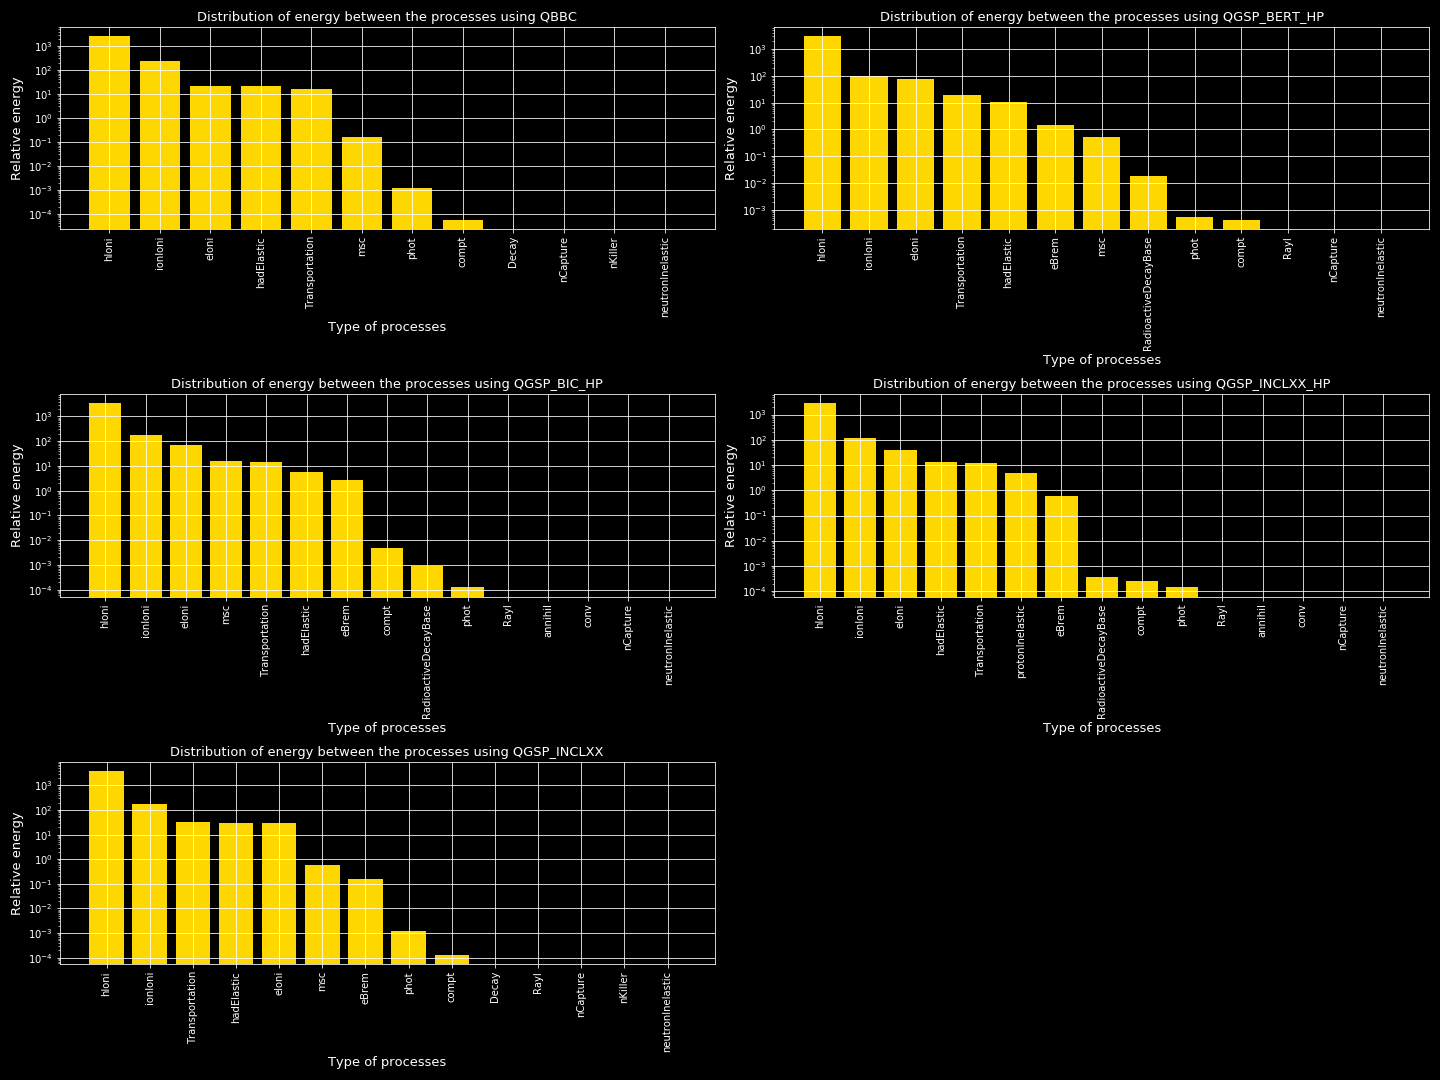
\includegraphics[scale = 0.28]{enproc.png}
    \caption{Summing the relative energy distributed among the particles by generating process.}
    \label{fig:my_label}
\end{figure}

\begin{figure}[H]
    \centering
    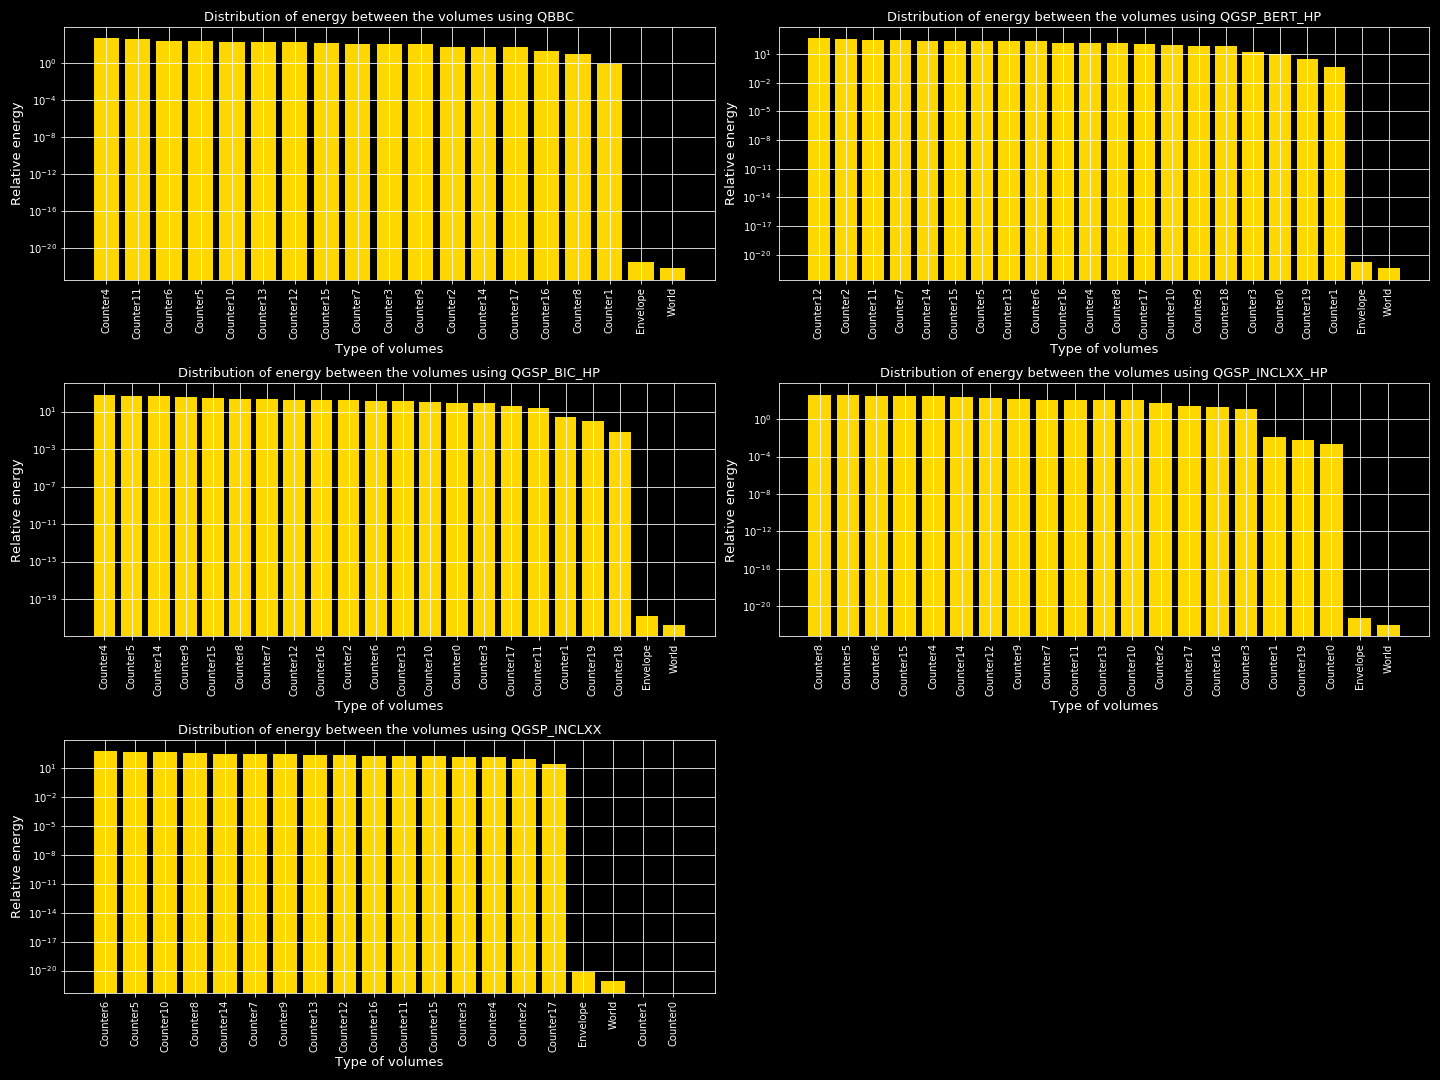
\includegraphics[scale = 0.27]{envol.png}
    \caption{Summing the relative energy distributed among the particles by the volumes they were detected in.}
    \label{fig:my_label}
\end{figure}

\end{document}
